\documentclass[10pt]{article}

%\mode<presentation>{}
\usepackage[left=1.2in,top=1.0in,right=.5in,bottom=1.0in,landscape]{geometry}
\usepackage[utf8]{inputenc}
\usepackage{graphicx}
\usepackage{tikz}
\usepackage{tcolorbox}
\usepackage[absolute,overlay]{textpos}
\usepackage{changepage}
\usepackage{xcolor}
%\tikzstyle{every node} = [align=center]
\usepackage{helvet}
%\usepackage{sansmathfonts}
\usepackage{amsmath}
\renewcommand{\familydefault}{\sfdefault}

\newcommand\BWone{3.5}
\newcommand\BWtwo{3}
\newcommand\BWthree{3}
\newcommand\BHone{0.5}
\newcommand\BHtwo{1}
\newcommand\BHthree{1.1}

\newcommand\Vgap{1}

\newcommand\Hone{-8}
\newcommand\Htwo{\Hone + \BWone + \BWone + \Vgap}
\newcommand\Hthree{\Htwo + \BWone + \BWone + \Vgap}

\newcommand\Vone{1}

\newcommand\Vtwo{-6}

\newcommand\Vthree{-8.3}

\newcommand\HGap{0.5}

\newcommand{\Upperbox}{.8}

\newcommand\Loffset{0.3}

\definecolor{boxcolor}{HTML}{fab71b}
\definecolor{title1}{HTML}{0070c0}
\definecolor{title2}{HTML}{2f5496}

\begin{document}

%\begin{frame}

\begin{adjustwidth}{-6em}{}

\begin{tikzpicture}
  \node[anchor=north ] at (\Hone-\BWone -\Loffset,\Vone+\BHone+1+\Loffset) {\Large a}; 
  \node[anchor=north] at (\Hone,\Vone-1.2) {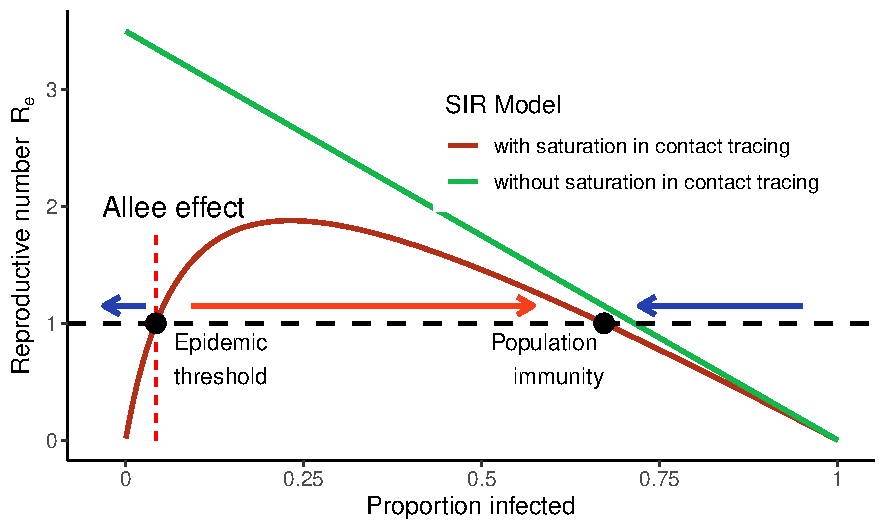
\includegraphics[scale=.45]{../allee1D.pdf}};
   \draw[fill = boxcolor, draw=none]  (\Hone-\BWone,\Vone ) rectangle (\Hone+\BWone,\Vone+\BHone)
   

       node[pos=0.5] {\scriptsize $R_e = P_{susceptible} \cdot b_{link} (L \cdot f_{q} + L_{max} \cdot f_{nq})$};

       \fill[title1] (\Hone-\BWone,\Vone+\BHone) rectangle (\Hone+\BWone,\Vone+\BHone+\Upperbox)
       node[pos=0.5,align=center,font=\scriptsize, color=white] {Non-pharmaceutical interventions (NPIs) \\ induce an Allee effect on disease dynamics};
;
\node[anchor=north ] at (\Htwo-\BWone -\Loffset,\Vone+\BHone+1+\Loffset) {\Large b}; 

       
  \fill[title2]  (\Htwo-\BWone,\Vone+\BHone) rectangle (\Htwo+\BWone,\Vone+\BHone+\Upperbox)
    node[pos=0.5,align=center,font=\scriptsize, color=white] {Transition between dynamic states is determined by the \\ strength of NPIs and the proportion of infected individuals};

  \node[anchor=north] at (\Htwo,\Vone+\BHone) {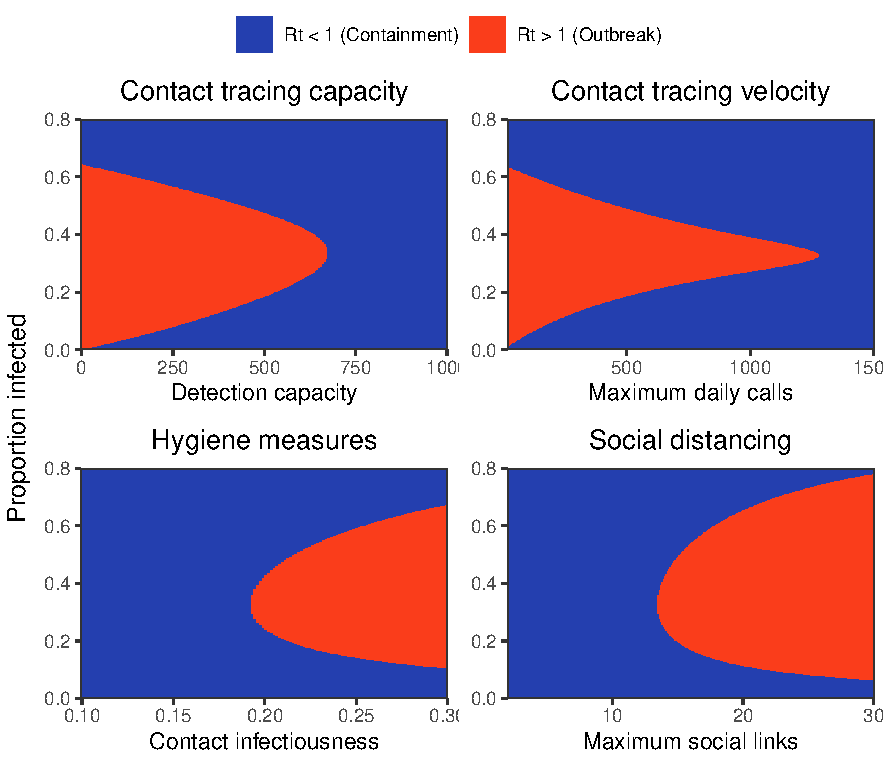
\includegraphics[scale=.45]{../phase_space.pdf}};

 \node[anchor=north ] at (\Hthree-\BWone -\Loffset,\Vone+\BHone+\Upperbox+\Loffset) {\Large c}; 

%   \fill[title2]  (\Hone-\BWone,\Vtwo-\BHone+1) rectangle (\Hone+\BWone,\Vtwo+1.8)
   \fill[title1] (\Hthree-\BWone,\Vone+\BHone) rectangle (\Hthree+\BWone,\Vone+\BHone+\Upperbox)
    node[pos=0.5,align=center,font=\scriptsize, color=white] {Simulated dynamics with an NPI-induced Allee effect \\ often show sharp accelerationsafter slow initial spread};

  
  \draw[fill=boxcolor,draw=none]  (\Hthree-\BWone,\Vone-\BHone) rectangle (\Hthree+\BWone,\Vone+\BHone)
    node[anchor=north east ,pos=1,align=left,font=\tiny] {\scalebox{0.6} \bf Simulated SIR Dynamics \\
    \begin{tabular}{l r}
       \scalebox{0.6} { $S(t+1) = S(t) - I_{new}(d)$ } & \scalebox{0.6} {$I_{new}(t)\sim {\rm Poisson}(\lambda) $ }\\
           \scalebox{0.6} {$I(t+1) = I(t) + I_{new}(t) - \frac{I(t)}{\gamma(I(t))} + I_{imp}(t) $  }  &  \scalebox{0.6}{ $\lambda= \frac{\beta(I(t)) I(t)^p S(t)}{N} $}\\
             \scalebox{0.6} {$R(t+1) = R(t) + \frac{I(t)}{\gamma(I(t))} $ } &   \scalebox{0.6} {$I_{imp}(t) \sim NB (\mu, \sigma) $} \\
  \end{tabular}\\

    
 };

  \node[anchor=north] at (\Hthree,\Vone-.8) {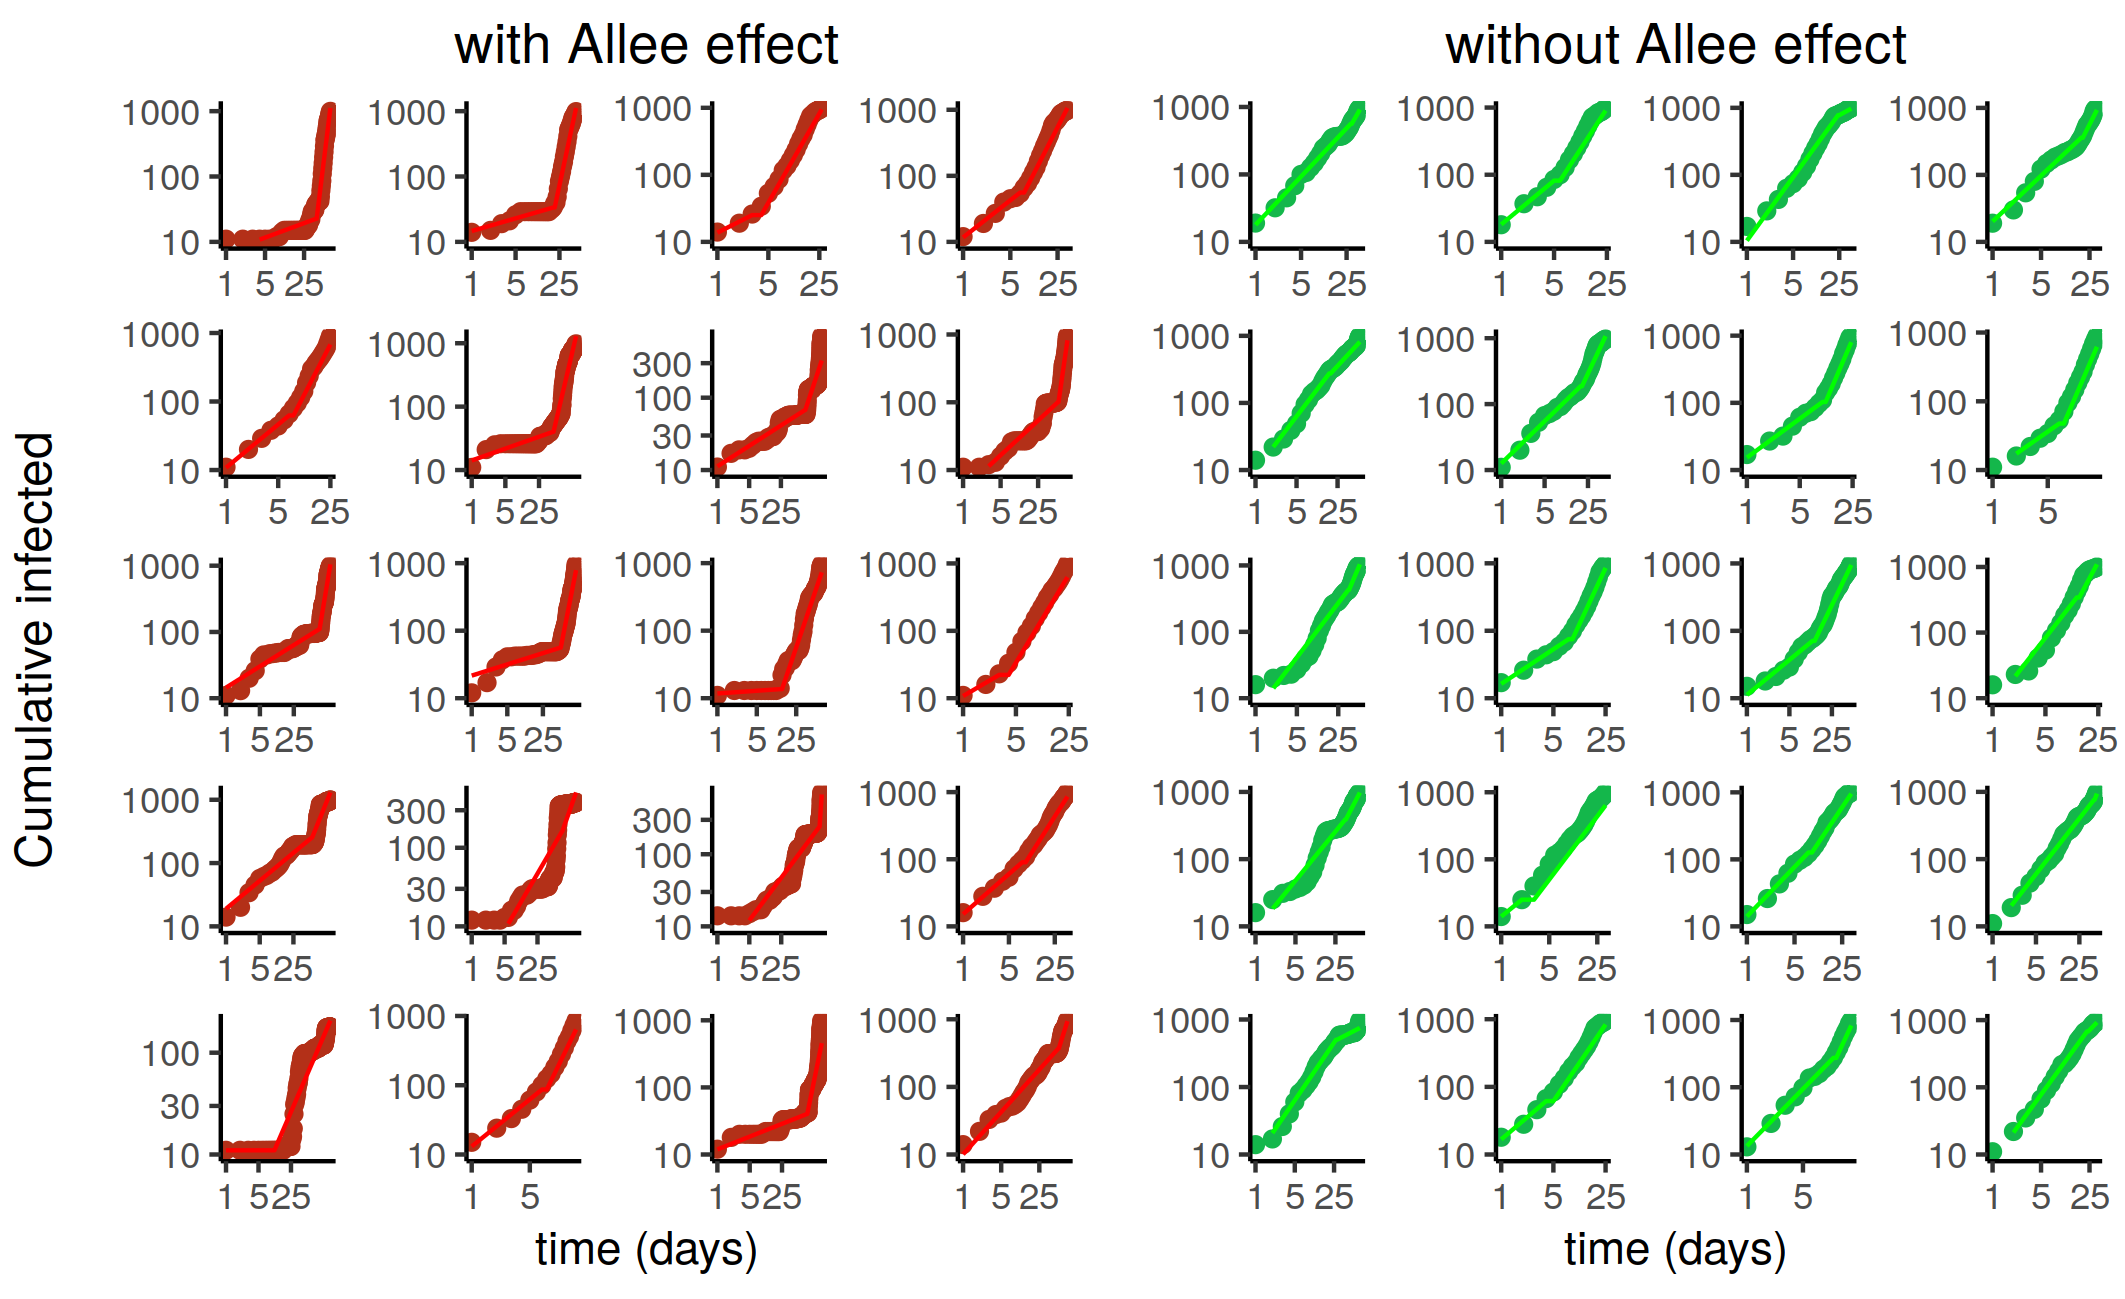
\includegraphics[scale=.4]{../simDynamics.png}};


\end{tikzpicture}

\end{adjustwidth}


\end{document}





